\paragraph*{Illustration: Gene/Protein regulatory network inference.}

As an illustration, we applied our sparse multiattribute GGM approach
to reconstruct networks on two large breast cancer data sets from the
National Cancer Institute\footnote{\url{https://www.cancer.gov/}} and
the Rational Therapy for Breast Cancer
consortium\footnote{\url{http://www.ratherproject.com/}}, respectively
referred to as NCI-60 and RATHER hereafter. These data sets contain
both proteomic and transcriptomic profiles, respectively measured with
reverse-phase protein arrays (RPPA) and RNA affymetrix array. We infer
the multiattribute network between the subset of molecular entities
which is common to the proteins measured by RPPA and the genes
measured by RNA array, that we call the \textit{consensus set}: in the
NCI-60 cancer line data set \citep{pfister2009topoisomerase}, a
consensus set composed of $p=91$ protein and corresponding gene
profiles is retained, for the $n=60$ samples. The RATHER data set
\citep{michaut2016integration} contains proteomic and transcriptonic
data from $n=100$ patients for a consensus set of $p=117$
entities\footnote{The data can be downloaded from
  \url{https://www.ncbi.nlm.nih.gov/geo/query/acc.cgi?acc=GSE66647}.}.

We infer a sparse GGM for each attribute (gene expression and protein
profile), separately to start with, and then get its multiattribute
version.  We do this on a large grid of the tuning parameter and thus
have three families of networks indexed by their number of edges.

Figure \ref{fig:jaccard} demonstrates that our sparse multiattribute
method captures the characteristics of both univariate networks, as
the Jaccard similarity index is high between each uni-attribute
network and the multiattribute network, while it remains low when
comparing uni-attribute networks together.
\begin{figure}[htbp!]
  \centering
  \begin{tabular}{@{}cc@{}}
   RATHER & NCI-60 \\
    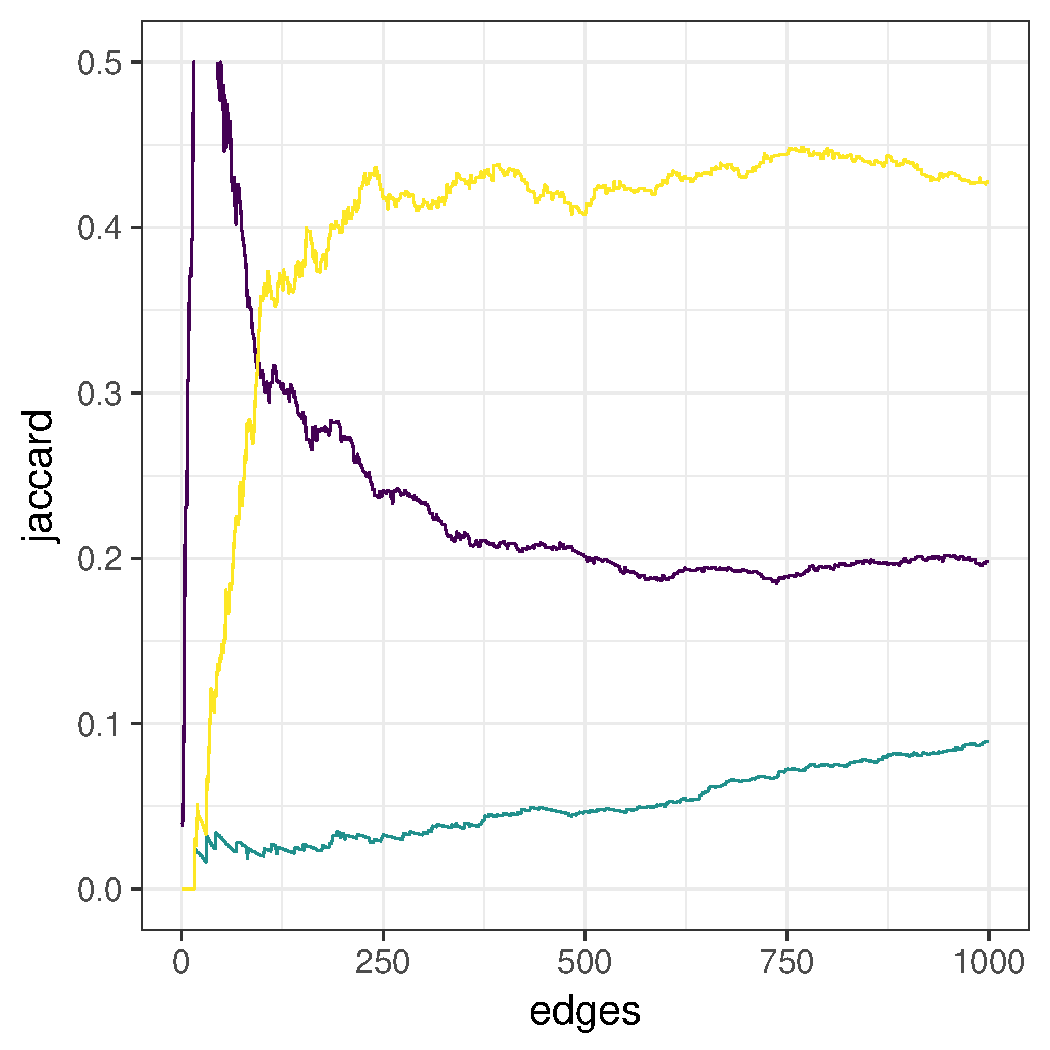
\includegraphics[width=.35\textwidth]{figures/jaccard_RATHER}
  & 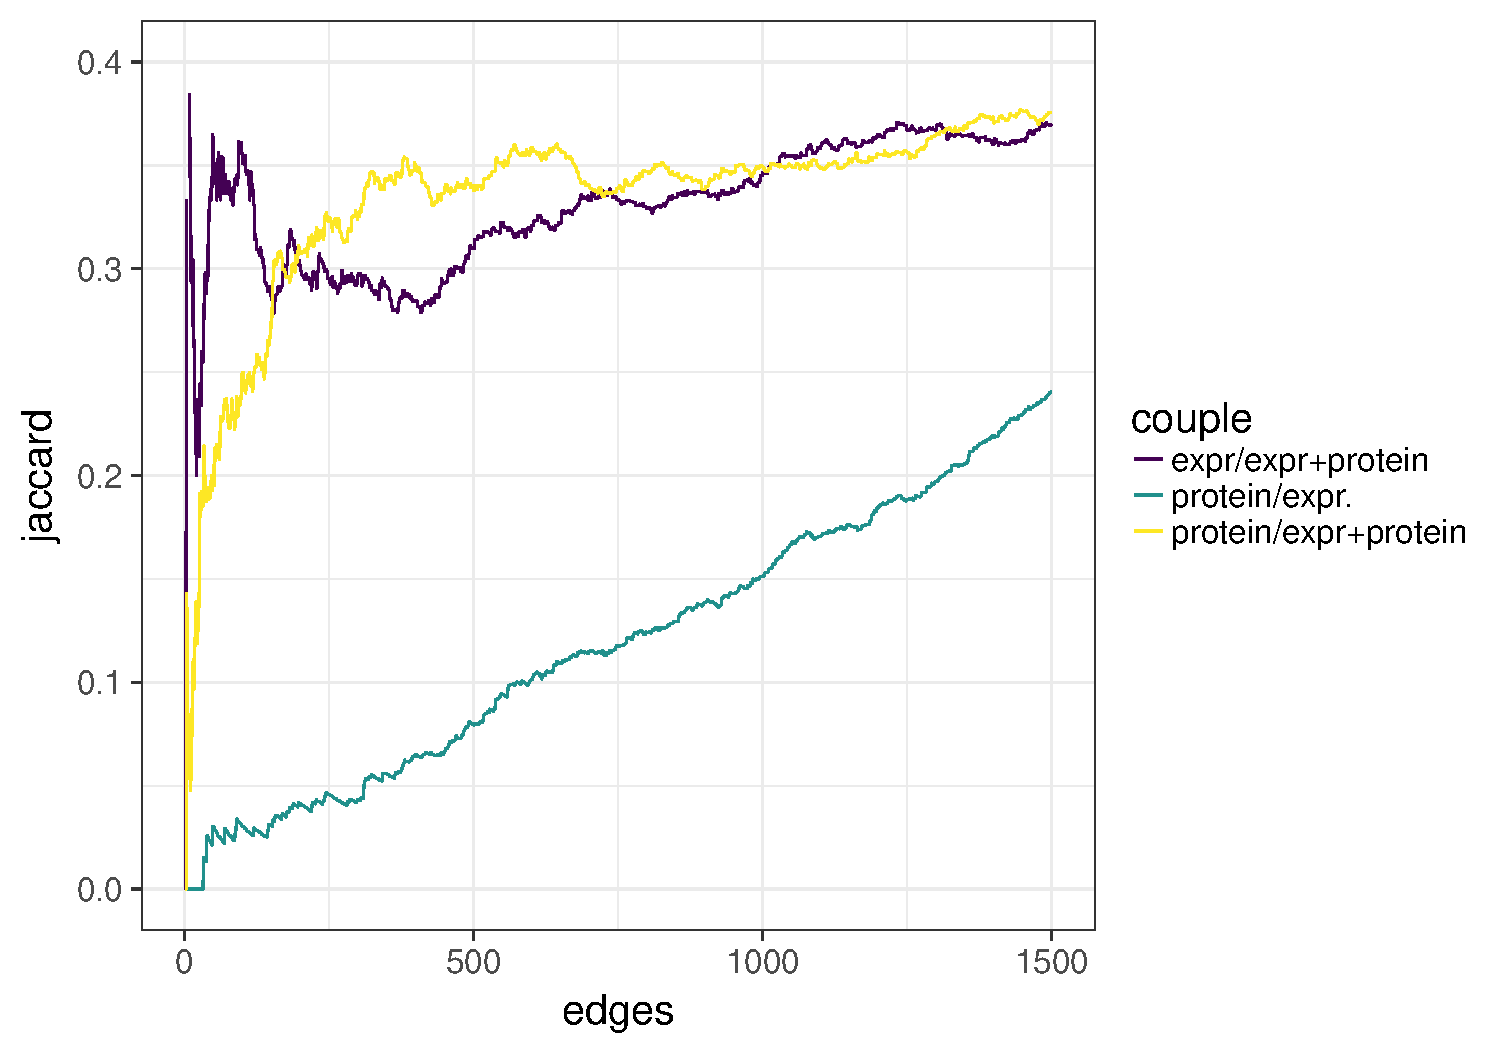
\includegraphics[width=.5\textwidth]{figures/jaccard_NCI60}
  \end{tabular}
  \caption{Jaccard's similarity index
    $J(A,B) = \frac{\left|A\cap B\right|}{\left|A\cup B\right|}$
    between uni-attribute and multiattribute networks, for RATHER and
    NCI60 data set: multiattribute networks share a high Jaccard
    index with both uni-attribute networks.}
  \label{fig:jaccard}
\end{figure}

Figure \ref{fig:networks} shows the finally retained networks, where
the number of edges is controlled by the tuning parameter $\lambda$
chosen by 10-fold cross-validation. It is clear that some motifs only
present in each uni-attribute networks are caught in their
multiattribute counterparts. This tends to prove that the
multiattribute version proposes a consensus version of the
interactions at hand in the cell, and one which is hopefully more
robust to noise.
\begin{figure}[htbp!]
  \centering
  \begin{tabular}{@{}lccc@{}}
    & proteomic network  & genomic network  & multiattribute network \\
    \rotatebox{90}{\hspace{1.2cm}NCI60} 
    & 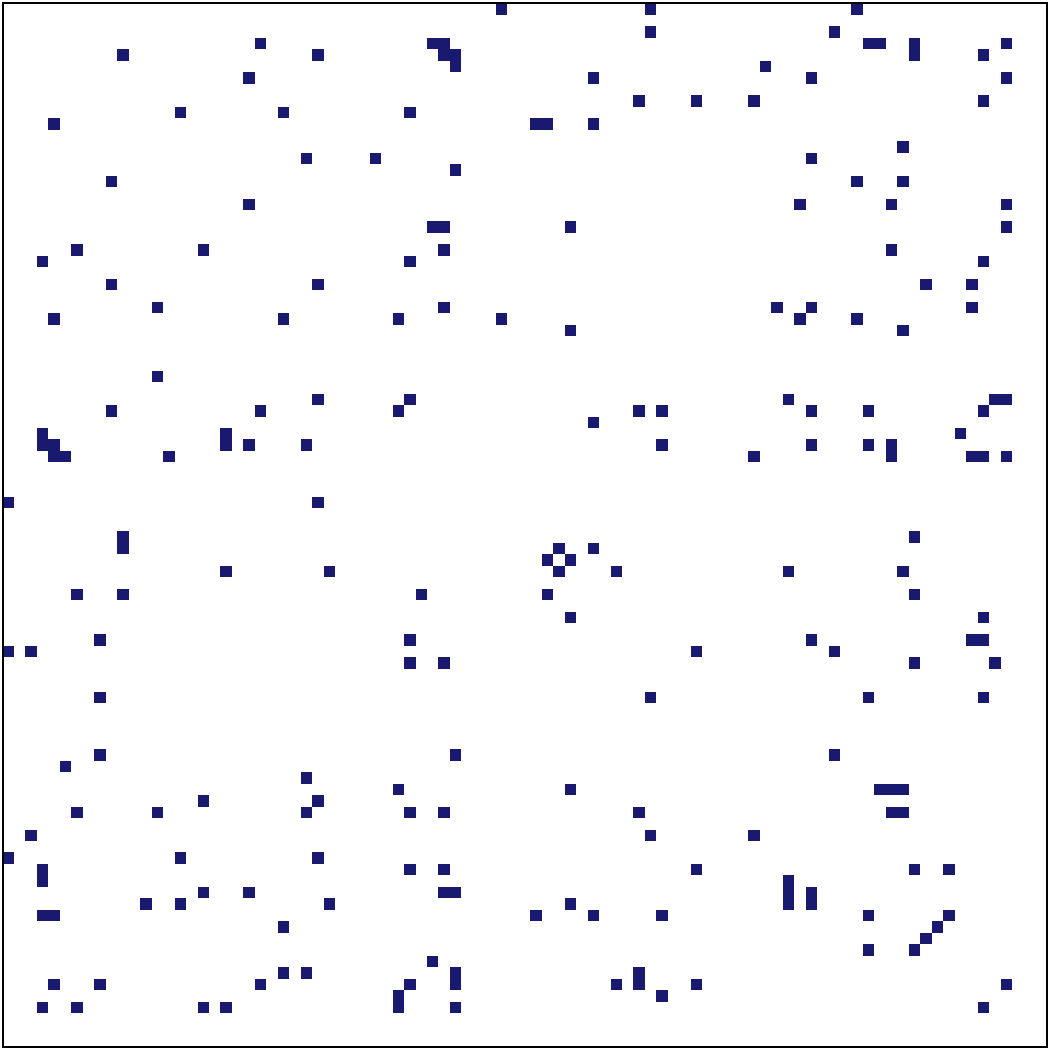
\includegraphics[width=.3\textwidth]{figures/protNet_NCI60}
    & 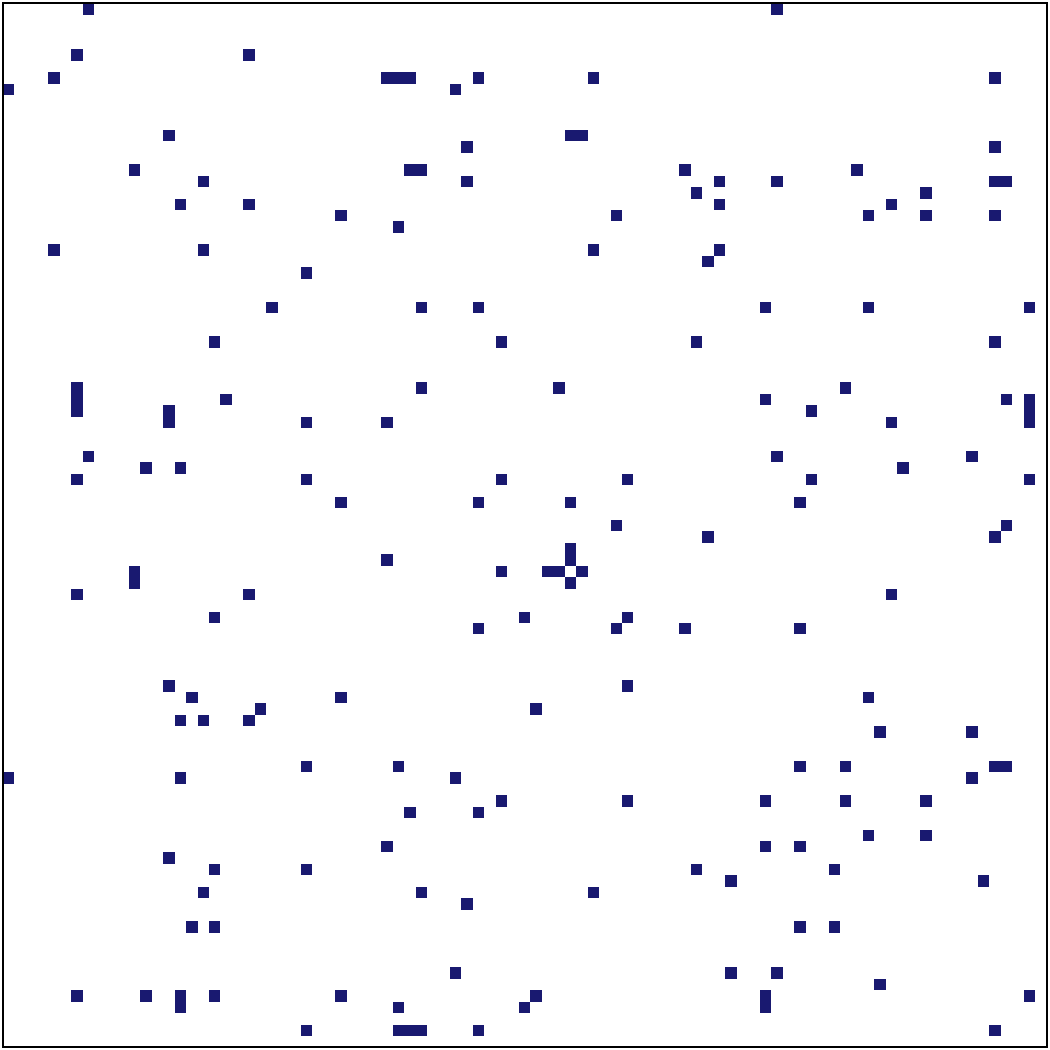
\includegraphics[width=.3\textwidth]{figures/exprNet_NCI60}
    & 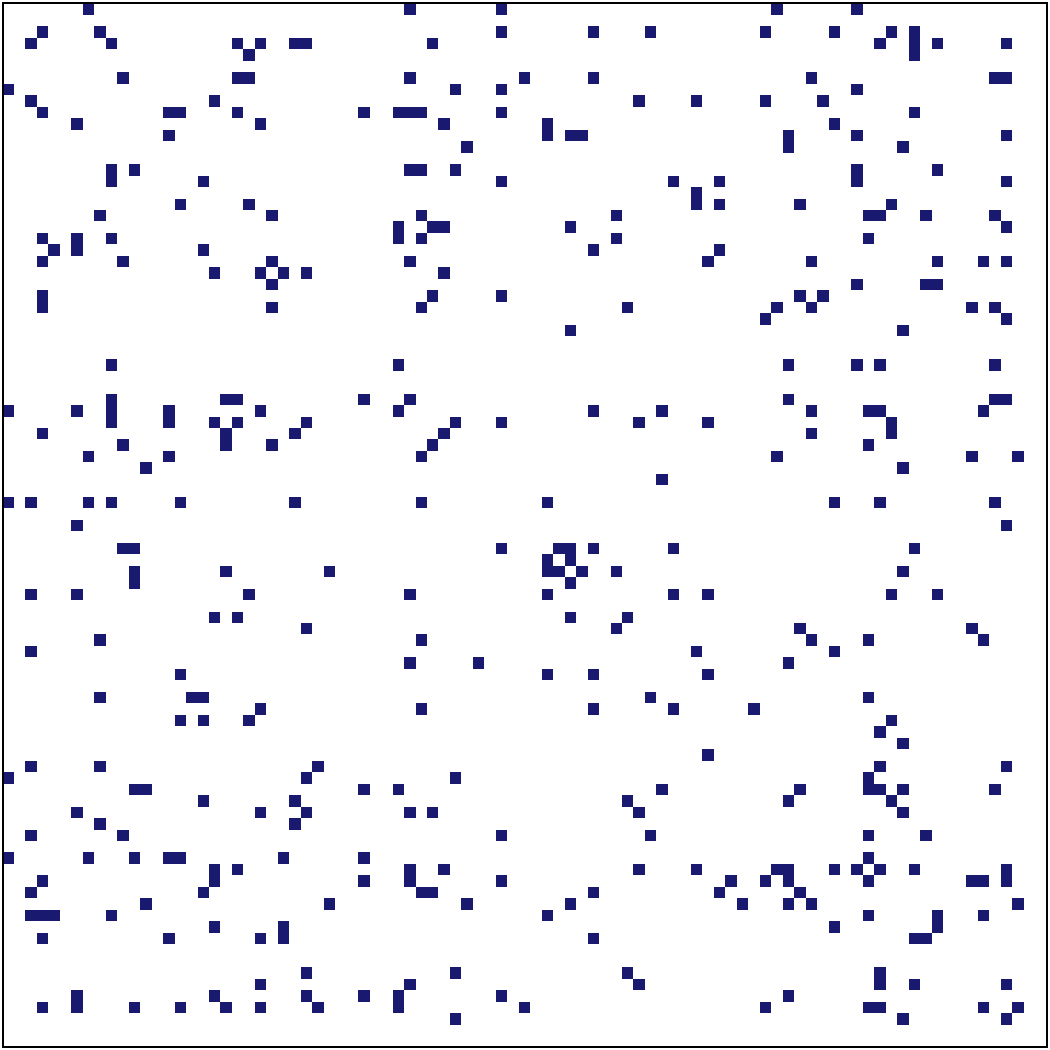
\includegraphics[width=.3\textwidth]{figures/bivarNet_NCI60} \\
    \rotatebox{90}{\hspace{1.2cm}RATHER} 
    & 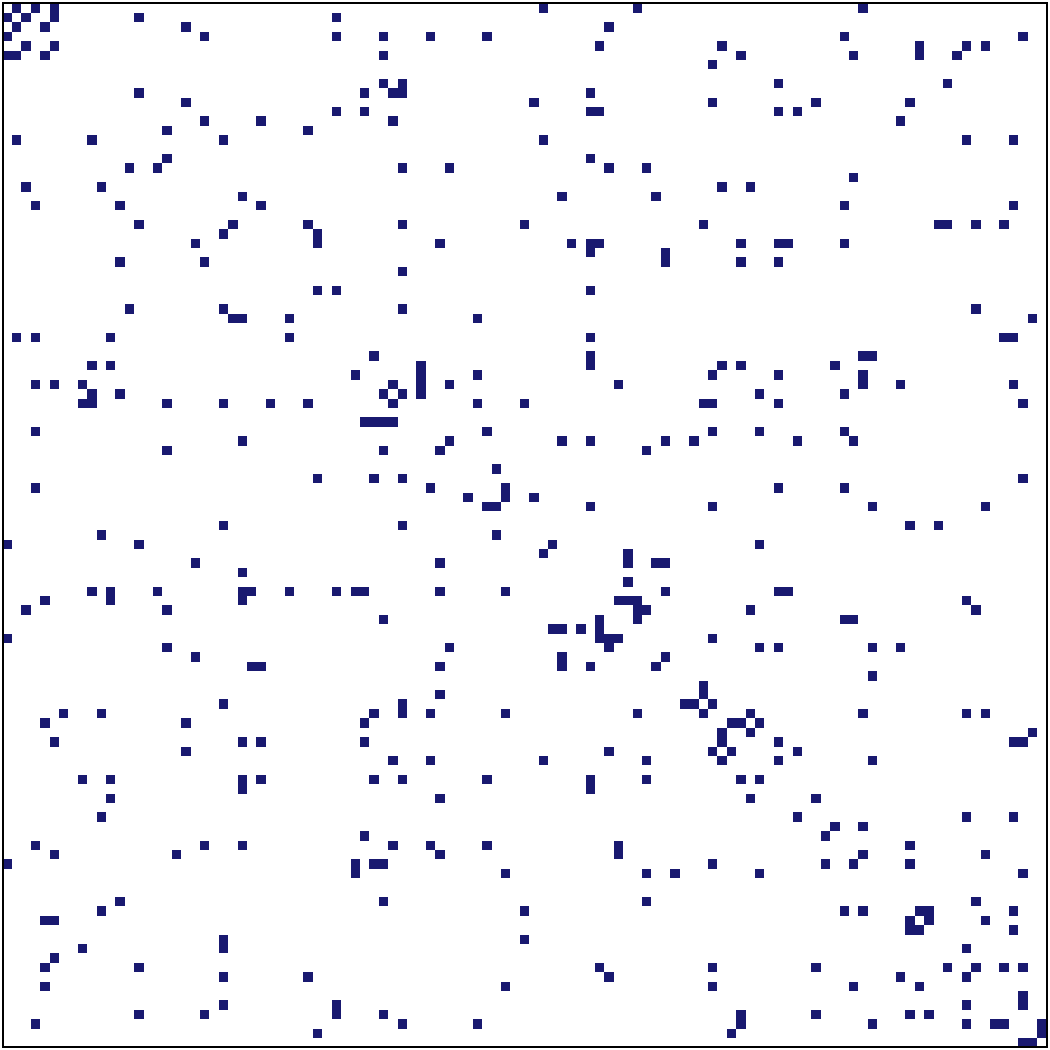
\includegraphics[width=.3\textwidth]{figures/protNet_RATHER}
    & 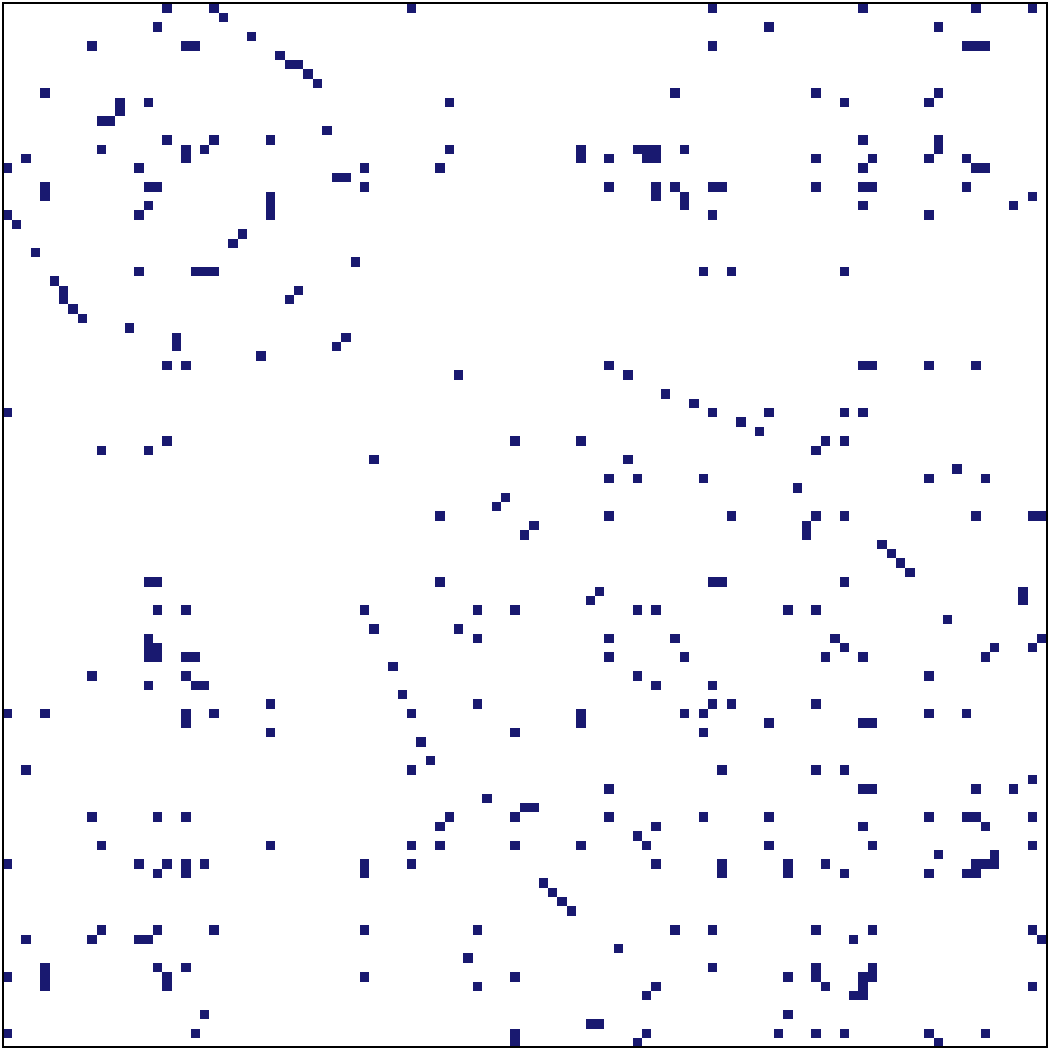
\includegraphics[width=.3\textwidth]{figures/exprNet_RATHER}
    & 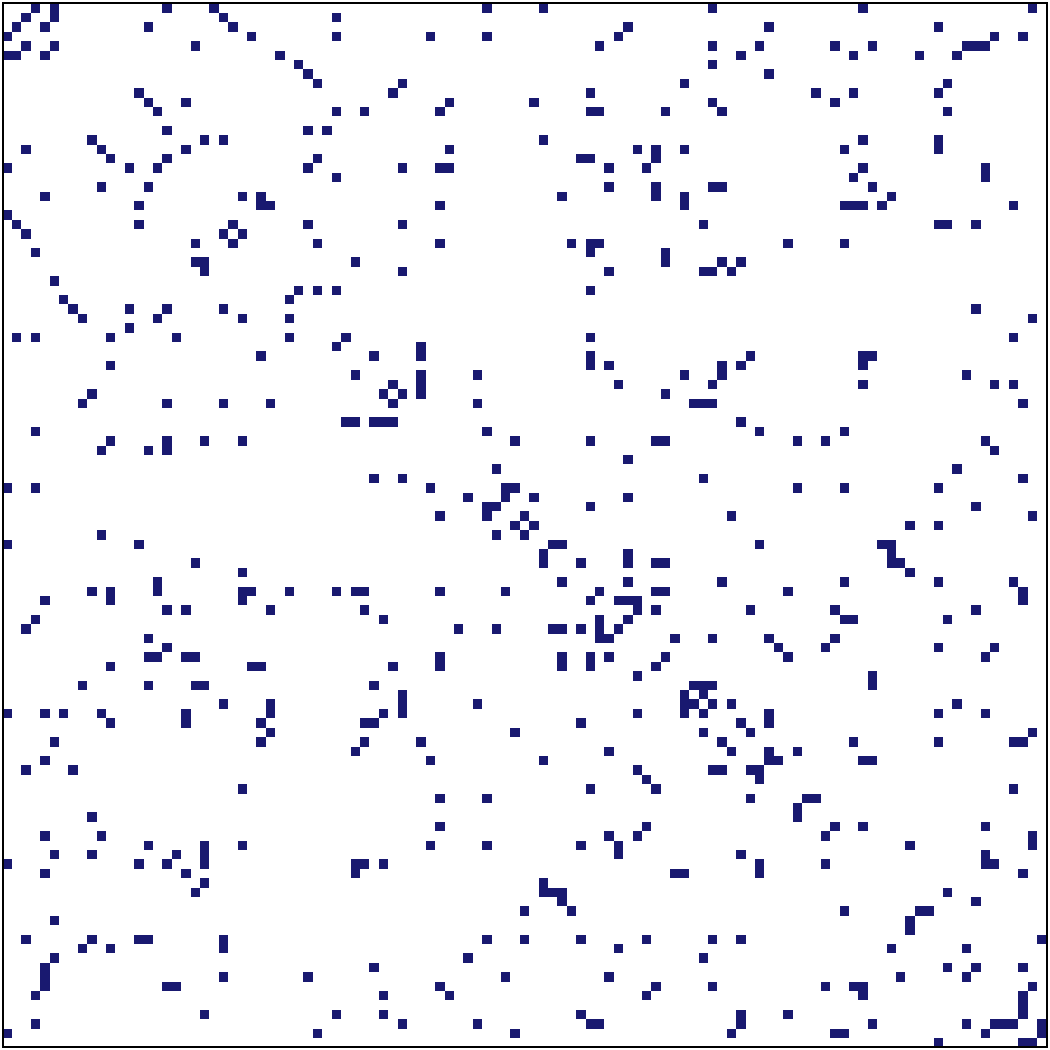
\includegraphics[width=.3\textwidth]{figures/bivarNet_RATHER} \\
  \end{tabular}
  \caption{Uni-attribute and multiattribute networks inferred on both
    NCI60 and RATHER dataset. The number of neighbors of each entity
    is chosen by cross-validation. Multiattribute networks catch motif
    found in the uniattribute counterparts.}
  \label{fig:networks}
\end{figure}



